\documentclass{article}

\usepackage{arxiv}

\usepackage[utf8]{inputenc} % allow utf-8 input
\usepackage[T1]{fontenc}    % use 8-bit T1 fonts
\usepackage{lmodern}        % https://github.com/rstudio/rticles/issues/343
\usepackage{hyperref}       % hyperlinks
\usepackage{url}            % simple URL typesetting
\usepackage{booktabs}       % professional-quality tables
\usepackage{amsfonts}       % blackboard math symbols
\usepackage{nicefrac}       % compact symbols for 1/2, etc.
\usepackage{microtype}      % microtypography
\usepackage{lipsum}
\usepackage{graphicx}

\title{A template for the \emph{arxiv} style}

\author{
    Derek Powell
   \\
    School of Social and Behavioral Sciences \\
    Arizona State University \\
  Phoenix, AZ \\
  \texttt{\href{mailto:dmpowell@asu.edu}{\nolinkurl{dmpowell@asu.edu}}} \\
  }


% Pandoc citation processing
\newlength{\csllabelwidth}
\setlength{\csllabelwidth}{3em}
\newlength{\cslhangindent}
\setlength{\cslhangindent}{1.5em}
% for Pandoc 2.8 to 2.10.1
\newenvironment{cslreferences}%
  {}%
  {\par}
% For Pandoc 2.11+
\newenvironment{CSLReferences}[3] % #1 hanging-ident, #2 entry spacing
 {% don't indent paragraphs
  \setlength{\parindent}{0pt}
  % turn on hanging indent if param 1 is 1
  \ifodd #1 \everypar{\setlength{\hangindent}{\cslhangindent}}\ignorespaces\fi
  % set entry spacing
  \ifnum #2 > 0
  \setlength{\parskip}{#2\baselineskip}
  \fi
 }%
 {}
\usepackage{calc} % for calculating minipage widths
\newcommand{\CSLBlock}[1]{#1\hfill\break}
\newcommand{\CSLLeftMargin}[1]{\parbox[t]{\csllabelwidth}{#1}}
\newcommand{\CSLRightInline}[1]{\parbox[t]{\linewidth - \csllabelwidth}{#1}}
\newcommand{\CSLIndent}[1]{\hspace{\cslhangindent}#1}

\usepackage{booktabs}
\usepackage{longtable}
\usepackage{array}
\usepackage{multirow}
\usepackage{wrapfig}
\usepackage{float}
\usepackage{colortbl}
\usepackage{pdflscape}
\usepackage{tabu}
\usepackage{threeparttable}
\usepackage{threeparttablex}
\usepackage[normalem]{ulem}
\usepackage{makecell}
\usepackage{xcolor}


\begin{document}
\maketitle

\def\tightlist{}


\begin{abstract}
Enter the text of your abstract here.
\end{abstract}

\keywords{
    blah
   \and
    blee
   \and
    bloo
   \and
    these are optional and can be removed
  }

\hypertarget{introduction}{%
\section{Introduction}\label{introduction}}

Bayesian theories of cognition have had remarkable successes in
explaining human reasoning and behavior across many domains (big cite).
{[}The core of these theories is that people reason according to
subjective mentally-represented degrees of belief, and they specify how
they should be revised in light of evidence. It is somewhat embarrassing
then that one area where these theories seem to fall down is in
describing human ``beliefs'\,' of the simple and everyday sort, such as
beliefs like''it will rain tomorrow``, ``vaccines are safe,'' or ``this
politician is trustworthy.''

Trouble starts as soon as we seek to measure beliefs. According to
Bayesian theories of cognition and epistemology, the degree to which
people believe in various propositions should reflect subjective mental
probabilities. So asking people to express beliefs in terms of
probability seems only natural.

Unfortunately, people's explicit probability judgments routinely violate
the axioms of probability theory. For example, human probability
judgments often exhibit the ``conjunction fallacy'': people will often
judge the conjunction of two events (e.g.~``Tom Brady likes football and
miniature horses'') as being more probable than one of the events in
isolation (e.g.~``Tom Brady likes miniature horses''), a plain and
flagrant violation of probability theory (cite some examples). Other
demonstrations of the incoherence of probability judgments include
disjunction fallacies (e.g.~XXX), ``unpacking'' effects (e.g.~fox \&
tversky), and a variety of other effects illustrating the incoherence of
human probability judgments {[}cite{]}. Altogether these findings have
led many researchers to abandon the notion that credences are
represented as probabilities.

Recently however, two groups of researchers have proposed theories of
human probability judgments that account for biases and apparent
incoherence in these judgments while maintaining that mental credences
are fundamentally probabilistic (Costello and Watts 2014; Zhu, Sanborn,
and Chater 2020). Both of these theories build on the increasingly
popular notion that a variety of human reasoning tasks are accomplished
by drawing a limited number of samples from probabilistic mental models
(see also Chater et al. 2020; Dasgupta, Schulz, and Gershman 2017).

\hypertarget{two-probabilistic-theories-of-probability-judgment}{%
\subsection{Two probabilistic theories of probability
judgment}\label{two-probabilistic-theories-of-probability-judgment}}

Costello \& Watts (2014, 2016, 2018) proposed a theory of probability
judgment they call the ``Probability Theory plus Noise'' theory (PT+N).
In the PT+N model, mental ``samples'' are drawn from a probabilistic
mental model of events and are then ``read'' with noise, so that some
positive examples will be read as negative and some negative read as
positive. This results in probability judgments that reflect
probabilistic credences perturbed by noise. Under the simplest form of
the PT+N model, the expected value of probability judgments is:

\[E[\hat{P}_{PT+N}(A)] = (1-2d)P(A) + d \]

where \emph{d} represents the probability with which samples will be
misread, or the amount of noise in the judgment process (where by
assumption a maximum of 50\% of samples can be misread, so that d is a
number in the range {[}0, .50{]}). The PT+N theory provides a unified
accounts for a wide variety of biases in probability judgment that were
previously attributed to different types of heuristics (Costello and
Watts 2014, 2016, 2017, 2018).

Meanwhile, Zhu, Sanborn, \& Chater (2020) have proposed a Bayesian model
of probability judgment they call the ``Bayesian Sampler.'' Under this
model, probability judgment is itself seen as a process of Bayesian
inference. To judge the probability of an event, a limited number of
samples are again drawn from a mental model of the event. Then, those
``observed'' samples are integrated with a prior over probabilities to
produce a probability judgment. The effect of this prior is to
regularize the judgments, pushing them away from extreme values. They
argue this regularization of judgments is adaptive, in that it pushes
judgments and decisions away from extremes that might, e.g.~encourage
taking large risks based on a small number of mental samples. However,
this hedging comes at the cost of systematic incoherence and biases.
Like the PT+N model, their proposed model accounts for a wide array of
biases in probability judgments, including the novel biases identified
by Costello and Watts (Costello and Watts 2014, 2016).

Under the simplest version of the Bayesian Sampler model, the expected
value of a probability judgment is given by the following formula:

\[E[\hat{P}_{BS}(A)] = \frac{N}{N+2\beta}P(A) + \frac{\beta}{N+2\beta}\]

where \emph{N} represents the number of mental samples drawn. The
mentally-observed samples are integrated with a Bayesian prior over
probabilities, represented with a symmetric beta distribution
parameterized by \(\beta\). Zhu and colleagues (2020) show that the
\emph{N} and \(\beta\) parameters of their model can be related to the
\emph{d} parameter of the PT+N model via the following bridging formula:

\[d = \frac{\beta}{N+2\beta}\]

\hypertarget{two-accounts-of-conditional-probability-judgments}{%
\subsubsection{Two accounts of conditional probability
judgments}\label{two-accounts-of-conditional-probability-judgments}}

By explaining the incoherence of human probability judgments using
coherent mental probabilities, both models have the potential to rescue
the larger project of Bayesian cognitive science as applied to everyday
beliefs (Chater et al. 2020). However, because they diverge in their
treatment of conditional probability judgments, the two theories fit
very differently into the larger Bayesian project. According to the
Bayesian sampler model, conditioning is something that happens in the
mental model of the events, not as part of the process of rendering
probability judgments. Thus, the Bayesian sampler model does not assign
any special status to conditional probability judgments and so fits
neatly into the larger Bayesian project of cognitive science:
probability judgments are simply another judgment process applied to the
outputs of other Bayesian mental models (Chater et al. 2020).

In contrast, the PT+N model presents a constructive account of
conditional probability judgments that is fundamentally non-Bayesian
(Costello and Watts 2016). According to the PT+N model, conditional
probabilities P(A\textbar B) are estimated by a two-stage sampling
procedure: first both events A and B are sampled with noise, and then a
second noisy process computes the ratio of the events read as A and B
over events read as B. The PT+N model predicts conditional probability
estimates using the following equation:

\[ P_e(A|B) = \frac{(1-2d)^2P(A \land B) + d(1-2d)\big(P(A)+P(B)\big)+d^2}{(1-2d)P(B)+d} \]\\
Given that conditional inference and belief updating lies at the core of
Bayesian cognitive theory, PT+N's account of conditional probability
judgment separates it from the Bayesian sampler theory not just
quantitatively, but quite fundamentally. First, it denies any central
importance of conditional probability judgments by pulling conditioning
out of the mental model of an event and placing it into the probability
judgment process. And perhaps more importantly, this non-bayesian
account of conditional inference can no longer be considered
``rational'' at any stage under the PT+N model.

\hypertarget{comparing-the-models}{%
\subsection{Comparing the models}\label{comparing-the-models}}

Zhu, Sanborn, and Chater (2020) compared their Bayesian Sampler model
against Costello \& Watts' (2014; 2016; 2017; 2018) PT+N model as
explanations for human probability judgments in two experiments.
Unfortunately, their results were somewhat equivocal. They fit both
``simple'' and ``complex'' versions of each model and computed a
Bayesian Information Criteria score (BIC) for all models. The complex
versions of these models introduce additional parameters d' and N' that
allow for different patterns of judgments for conjunctive and
disjunctive judgments as compared with simple probability judgments.
These additional parameters are needed in order to explain conjunction
fallacies (Costello \& Watts, 2017; Zhu et al., 2020). Table 1 below
presents the total BIC scores computed for each model as originally fit,
using the authors' original code and saved model outputs (Zhu et al,
2020, Supplementary materials).

\begin{table}

\caption{\label{tab:table1}Original model fitting results}
\centering
\begin{tabular}[t]{lrr}
\toprule
Model & Exp. 1 & Exp. 2\\
\midrule
Bayesian Sampler simple & 956.9 & -5371.9\\
Bayesian Sampler complex & 1174.4 & -5099.3\\
PT+N simple & 1257.5 & -4901.1\\
PT+N complex & 1039.7 & -5159.6\\
Bayesian Sampler avg. & 1065.6 & -5235.6\\
\addlinespace
PT+N avg. & 1148.6 & -5030.4\\
\bottomrule
\end{tabular}
\end{table}

In both experiments, the simple version of the Bayesian Sampler scores
best, but the complex version of the PT+N model comes in second (lower
BIC scores are better). It is not obvious what conclusions should be
drawn from these results. Of course, the simple Bayesian Sampler model
appears to win by the numbers. But conjunction fallacies are an
extremely robust empirical finding (e.g.~cite) and are clearly present
in the data collected by Zhu and colleagues (2020). So we might rule out
the simple variants of the models on the grounds that they will fail to
capture important qualitative features of the data, which would instead
favor the PT+N theory. For their part, Zhu and colleagues (2020) elect
to split the baby by averaging the simple and complex model scores
together. This approach somewhat favors the Bayesian Sampler theory
overall, though they are rightfully cautious about drawing any strong
conclusions.

\hypertarget{accounting-for-model-complexity}{%
\subsubsection{Accounting for Model
Complexity}\label{accounting-for-model-complexity}}

Zhu and colleagues (2020) warn that BIC, which penalizes models based
only on the number of parameters in the model, cannot fully account for
the differences in the models' complexity. There are at least three
challenges to accounting for model complexity in the comparison of these
models. First, the models differ not only in the number of parameters
but in the domain of those parameters. Zhu and colleagues (2020)
restrict the range of the \(\beta\) parameter in their Bayesian Sampler
model to fall within the interval {[}0,1{]}. This restriction constrains
the Bayesian Sampler model's prior distribution to the class of
``ignorance priors,'' symmetric beta distributions where \(\beta < 1\).
Via the bridging conditions (eq X), they show that this restricts the
``noise level'' for the Bayesian Sampler, represented in implied d under
the PT+N model, to {[}0, \(\frac{1}{3}\){]} whereas the PT+N model
permits noise values between {[}0, 0.50{]}.

Second, it is not immediately clear how the structural differences
between the models impact their flexibility. For the purposes of model
comparison, the ``complexity penalty'' that models truly ought to pay is
determined by their relative flexibility in accommodating different
patterns of data, not simply the number or domain of their parameters
(cite Gelman). To be sure, Zhu and colleagues' (2020) bridging condition
makes it clear that the PT+N model is more flexible when it comes to
predicting unconditional probabilities. But, what impact does the PT+N
model's treatment of conditional probabilities have on model complexity?
Is this component of the model a sort of Ptolemaic epicycle, adding
complexity to the model that should be penalized? Or, does it constitute
a commitment to novel predictions that thereby constrain its
flexibility? Determining model complexity a priori is not always
straightforward when the models being compared differ structurally.

Finally, one potential explanation for the relative weakness of the
complex model versions is Zhu and colleagues' (2020) use of unpooled
models, where parameters are estimated independently for each individual
participant. Adding a parameter for each participant may effectively
over-penalize the ``complex'' variants relative to the simple variants,
especially if there is actually limited heterogeneity across
participants. In contrast, a comparison of fully pooled variants of the
simple and complex models (where a single population parameter is used
for all participants) would require adding only one extra parameter to
the penalty term. Partial pooling is a solution that balances between
these extreme approaches, allowing for an accounting of heterogeneity
without over-penalizing in cases where heterogeneity is low.

\hypertarget{the-present-work}{%
\subsubsection{The present work}\label{the-present-work}}

Here, I cast both the Bayesian Sampler and PT+N models into a Bayesian
data analysis framework that permits a more decisive (or at least
alternative) comparison. A Bayesian analysis allows issues of model
complexity to be addressed through comparisons of model fit based on
information criteria, such as WAIC and LOO\textsubscript{ic}. These
indices allow for complexity penalties that directly capture differences
in the flexibility of the models, rather than being estimated based
solely on the number of distinct parameters {[}cite gelman{]}. In
addition, this framework also supports straightforward implementation of
hierarchical versions of these models with partial pooling. This allows
for information about model parameters to be shared across participants,
resulting in an overall reduction in model complexity and a more
realistic test of the models.

\hypertarget{methods}{%
\section{Methods}\label{methods}}

\hypertarget{data-selection}{%
\subsection{Data selection}\label{data-selection}}

Zhu, Sanborn, \& Chater (2020) conducted two experiments to compare the
PT+N and Bayesian sampler theories. These experiments asked participants
to judge the probability of different events in various combinations.
Following prior work by Costello and Watts (e.g. 2016, 2018), both
experiments focused on the everyday events of different kinds of
weather.

Experiment 1 asked about the events \{icy, frosty\} and \{normal,
typical\} (e.g.~``what is the probability that the weather in London is
normal and not typical?''). The authors' goal was to ask about highly
correlated events, but the events used are perhaps nearly perfectly
correlated. Because the terms used to describe these events are nearly
synonymous, there is a concern about the interpretation of the
statements evaluated in this experiment. This is especially clear, as
the authors note, for disjunctive trials such as ``normal or typical,''
where ``or typical'' might not be read as a disjunction but rather an
elaborative clause. In light of these concerns, I excluded the
disjunctive trials from Experiment 1 from my analyses. Experiment 2
focused on more moderately correlated events, \{cold, rainy\} and
\{windy, cloudy\}, that do not admit these misinterpretations. In
addition, a third experimental condition asking about \{warm, snowy\}
was also included in the experiment, but was dropped from the analyses
reported in the paper. Exploring the raw responses from this condition
reveals a substantial fraction of ``zero'' and ``one'' responses for
certain trials. This may reflect a different response process than was
intended. For instance, some participants may have engaged in deductive
reasoning to judge that it is not possible for the weather to at once be
warm and snowy, and therefore responded with zero---failing to properly
consider that it is possible (at least logically) for it to be warm and
snowy at different times within the same day. Given these potentially
aberrant responses, I followed Zhu and colleagues (2020) in ignoring
data from this condition.

\hypertarget{modeling}{%
\subsection{Modeling}\label{modeling}}

I implement both the Bayesian Sampler and PT+N models as Bayesian models
in the probabilistic programming language Numpyro. All code and results
are available as supplemental materials
(\url{https://github.com/derekpowell/bayesian-sampler}).

\hypertarget{bayesian-implementations-of-the-models}{%
\subsubsection{Bayesian implementations of the
models}\label{bayesian-implementations-of-the-models}}

The PT+N model defines probability judgments as

\[P_{e}(A) = (1-2d)P(A) + d\]
\[P_e(A\land B) = (1-d^\prime)P(A \land B)+d^\prime\]
\[P_e(A\lor B) = (1-d^\prime)P(A \lor B)+d^\prime\]
\[P_e(A|B) = \frac{(1-2d)^2P(A \land B) + d(1-2d)\big(P(A)+P(B)\big)+d^2}{(1-2d)P(B)+d}\]

In contrast, the Bayesian Sampler model defines probability judgments as

\[P_{e}(A) = \frac{N}{N + 2 \beta}P(A) + \frac{\beta}{N+2 \beta}\]
\[P_{e}(A \land B) = \frac{N’}{N’ + 2 \beta}P(A \land B) + \frac{\beta}{N’+2 \beta}\]
\[P_{e}(A \lor B) = \frac{N’}{N’ + 2 \beta}P(A \lor B) + \frac{\beta}{N’+2 \beta}\]

Fixing d and d' or N and N' equal yields the ``simple'' variant of each
of the models, which treat conjunctive and disjunctive probability
judgments identically to simple probability judgments.

Notice that for each model the probability judgments depend on
underlying subjective probabilities, derived from a mental sampling
process. These subjective probabilities are unobserved, and must be
estimated as a latent variable. Here, they are estimated as a
four-dimensional dirichlet distribution for each subject, representing
the probability of the elementary events (A\&B, \textasciitilde A\&B,
A\&\textasciitilde B, \textasciitilde A\&\textasciitilde B).

Zhu, Sanborn \& Chater (2020) implement completely unpooled models with
separate d, d', N, N', and \(\beta\) parameters for each participant.
Translated into a Bayesian Framework, we can write the PT+N model as:

\[y_{ij} \sim beta\big(\mu_{ij} k, (1-\mu_{ij})k\big)\]
\[\mu_{ij} = f_{PT+N}(p_i, d_j, d_j) \]
\[ d_j = \frac{expit(\delta_j)}{2}\]
\[ d_j’ = \frac{expit\big(\delta_j + \exp(\Delta\delta_j)\big)}{2}\]
\[ p_i \sim Dirichlet(\overrightarrow{1})\]
\[ \delta_j \sim Normal(0,1)\] \[ \Delta\delta_j \sim Normal(0,1)\]
\[ k \sim HalfCauchy(20)\]

The function \(f_{PT+N}\) computes the expected probability estimate
using the underlying subjective probability p, the noise parameters d
and d', and the relevant equation as defined by the PT+N theory (see
supplemental materials for implementation details). Prior predictive
checks were conducted for all models to select priors that would be
uninformative or minimally informative on the scale of the model
parameters d and d'.

Recall that Zhu and colleagues (2020) identified a bridging condition
relating b and N in the Bayesian Sampler model to the d parameter of the
PT+N model. To support direct comparisons of the models, I parameterize
the Bayesian Sampler model according to the implied d and d', rather
than directly according to its \(\beta\), N, and N' parameters. I
constrain d to {[}0, \(\frac{1}{3}\){]} for the Bayesian Sampler model
to reflect the assumption that \(\beta \in [0, 1]\). This allows the
same priors to be used for the corresponding Bayesian Sampler and PT+N
models, simplifying their comparison.

The Bayesian Sampler model is therefore:

\[y_{ij} \sim beta\big(\mu_{ij} k, (1-\mu_{ij})k\big)\]
\[\mu_{ij} = f_{BS}(p_i, d_j, d_j’) \]
\[ d_j = \frac{expit(\delta_j)}{2}\]
\[ d_j’ = \frac{expit\big(\delta_j + \exp(\Delta\delta_j)\big)}{2}\]
\[ p_i \sim Dirichlet(\overrightarrow{1})\]
\[ \delta_j \sim Normal(0,1)\] \[ \Delta\delta_j \sim Normal(0,1)\]
\[ k \sim HalfCauchy(20)\]

Where the function \(f_{BS}\) computes the expected probability estimate
as prescribed by the Bayesian Sampler theory.

\hypertarget{hierarchical-implementations-of-the-models}{%
\subsubsection{Hierarchical implementations of the
models}\label{hierarchical-implementations-of-the-models}}

Both of these models can also be implemented as hierarchical models with
partial pooling for the d and d' parameters (implicitly, for N and N' in
the case of the Bayesian Sampler). This should prevent over-penalizing
complex versions of the model, as well as potentially improving their
overall predictive fit. The hierarchical implementation adds parameters
for the population-level d and d' as well as a parameter controlling the
standard deviation of the distribution for the subject-level effects.
For ease of interpretation, the centered parameterization is shown
below, although the actual models used a non-centered parameterization
to improve sampling efficiency (citation?).

\[y_{ij} \sim beta\big(\mu_{ij} k, (1-\mu_{ij})k\big)\]
\[\mu_{ij} = f_{BS}(p_i, d_j, d_j’) \]
\[d_j = \frac{ expit(\delta_j )}{3}\]
\[ d_j’ = \frac{ expit\big( \delta_j  + \exp(\Delta\delta_j )\big) }{3}\]
\[ p_i \sim Dirichlet(\overrightarrow{1})\]
\[ \delta_{pop} \sim Normal(-1, 1)\]
\[ \Delta\delta_{pop} \sim Normal(0, .50)\]
\[ log(\sigma_{\delta}) \sim Normal(-1, 1)\]
\[ log(\sigma_{\Delta\delta}) \sim Normal(-1, 1)\]
\[\delta_j \sim Normal(\delta_{pop}, \sigma_{\delta})\]
\[\Delta\delta_j \sim Normal(\Delta\delta_{pop}, \sigma_{\Delta\delta})\]
\[k \sim HalfCauchy(20)\]

Finally, I also explored fitting versions of the Bayesian Sampler model
that allowed values of \(\beta > 1\). Restricting \(\beta\) to {[}0,1{]}
restricts the prior distribution of the Bayesian sampler to the class of
``ignorance priors'' (Zhu et al., 2020). However, it is also possible
that people bring informative priors to the probability judgment task.
Indeed, Zhu and colleagues (2020) acknowledge there are situations where
an informative prior may be warranted (see e.g., Fennel \& Baddeley,
2012). If \(\beta\) is unrestricted, allowed to fall in the domain {[}0,
\(\infty\){]} then the Bayesian Sampler model becomes more flexible,
allowing for equivalent ``noise'' levels in the same {[}0, .50{]} range
as the PT+N model. Though it would seem a more fundamental change, this
model may also be seen as a version of the PT+N theory that jettisons
its constructive account of conditional probability judgment. Thus,
fitting this additional ``hybrid'' model allows for a complete
comparison of the models along both of their differing dimensions.

\hypertarget{results}{%
\section{Results}\label{results}}

I fit each of the models specified above to data from Zhu et al's (2020)
Experiment 1 and 2 and computed LOO\_ic scores for each combination.
Model posteriors were estimated using the Numpyro implementation of the
No-U-Turn Hamiltonian Markov chain Monte Carlo (MCMC) sampler (cite).
For each model, four MCMC chains of 2000 iterations were sampled after
2000 iterations of warmup and all passed convergence tests according to
\(\hat{R}\). Figure X below displays the estimated differences in
LOO\_ic scores for each of the models as compared to the best-scoring
model.

\begin{figure}[ht]
\centering
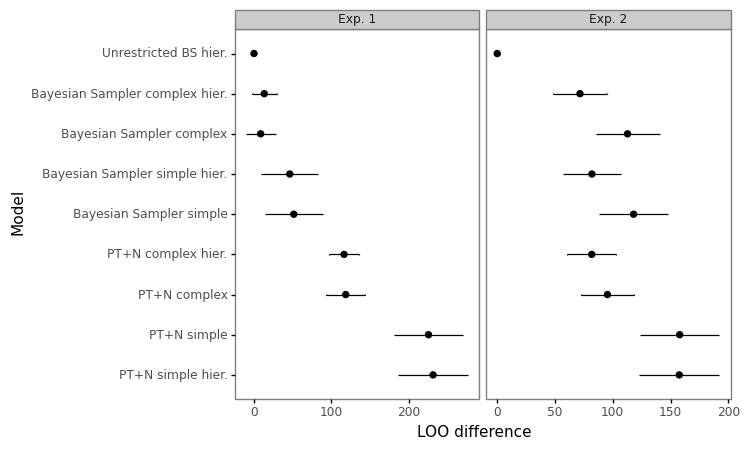
\includegraphics[width=5in]{plot_compare.png}
\end{figure}

Data from Experiment 1 are only modestly informative with respect to
discriminating among the models. However, data from Experiment 2 reveal
a clearer winner: a hierarchical implementation of the ``hybrid''
Bayesian Sampler model that removes the restriction on \(\beta\),
allowing it to range from {[}0, \(\infty\){]}.

Recall, this model may also be seen as a version of the PT+N theory that
removes the original theory's constructive account of conditional
probability judgments. Comparing predictions for conditional probability
judgments from the hybrid model and the best-fitting PT+N model, we see
that the hybrid model better captures these judgments from Experiment 2
(trial-average-level \(R^2\) = .85 vs .73; participant-level \(R^2\) =
.51 vs .45). These findings suggest that conditioning is better seen as
part of the mental model than the probability judgment process.

Figure X shows the posterior distributions of the population-level d and
d' parameters inferred from the ``hybrid'' model. Using data from
experiment 2, population-level estimates of d and d' are greater than
\(\frac{1}{3}\), outside the range implied by the assumption of
``ignorance priors'' in the Bayesian Sampler model. Parameters fit to
the data from Experiment 1 are more consistent with this assumption,
although a substantial proportion of of individual participants' d and
d' estimates also lie outside this range (13 of 59 for d, 26 of 59 for
d').

\begin{figure}[ht]
\centering
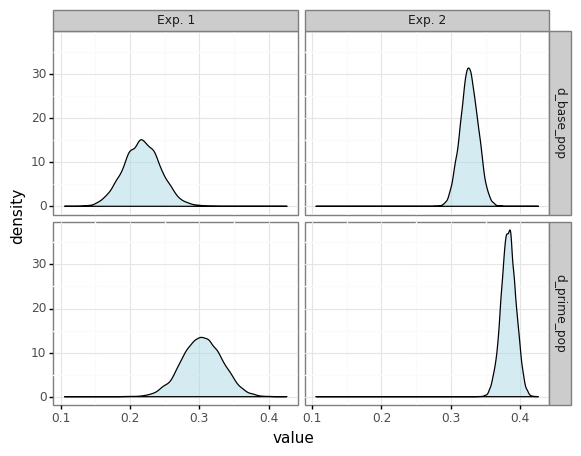
\includegraphics[width=4in]{plot_params.png}
\end{figure}

Among the remaining models, hierarchical implementations with partial
pooling outperform the unpooled corresponding models---suggesting that
unpool variants of the complex models were over-penalized in the
original analysis by Zhu, Sanborn, and Chater (2020). In both
experiments, the simple version of the PT+N model is clearly
outperformed by the other competing models. However, differences among
the remaining three models are approximately within the error of the
LOO\_ic estimates. As expected, the simple variants of the models have
smaller penalty terms than the complex variants.

Compared to the hybrid model, the PT+N model with its constructive
account of conditional probability judgments has a smaller penalty term
despite having the same parameterization in terms of d and d'. Evidently
this structural component isn't a complexifying epicycle, instead it is
a prediction that constrains flexibility. However, it is one that
ultimately leads to a worse-fitting model.

Perhaps surprisingly, the Bayesian Sampler with unrestricted beta
actually receives a smaller penalty term than the more restricted
version of the model. This is at first unintuitive, but it illustrates
how model complexity depends not only on the model and priors, but also
the observed data (see Gelman, Hwang, and Vehtari 2014). Gelman and
colleagues consider a case where a parameter is constrained to be
positive and its value is estimated from data (2014). If the estimated
value is some very large positive number, then the constraint won't have
been very informative. But, if the estimated value is very close to
zero, then the constraint that the parameter is positive will provide
substantial information and the model's penalty term will therefore be
smaller. Here, it seems reasonable to conjecture that because the
implied d and d' estimated for this data under this model are both very
near \(\frac{1}{3}\), the restriction results in posterior estimates of
the linear parameters that are relatively far from the prior, which can
result in a greater penalty.

The dependence of complexity penalties on observed data may strike some
as an undesirable feature of model comparison through information
criteria. Indeed, it is worth acknowledging that principled model
comparison is still an area of active inquiry, with differing
perspectives (e.g. Gronau and Wagenmakers 2019; Vehtari et al. 2019).
Fortunately, conclusions from the comparisons here do not rest solely on
differences between the models' complexity.

\begin{table}

\caption{\label{tab:table2}Bayesian model comparison results}
\centering
\begin{tabular}[t]{lrrrrrrrr}
\toprule
\multicolumn{1}{c}{ } & \multicolumn{4}{c}{Experiment 1} & \multicolumn{4}{c}{Experiment 2} \\
\cmidrule(l{3pt}r{3pt}){2-5} \cmidrule(l{3pt}r{3pt}){6-9}
Model & $LOO_{ic}$ & Penalty & $r_{resp}$ & $r_{trial}$ & $LOO_{ic}$ & Penalty & $r_{resp}$ & $r_{trial}$\\
\midrule
Unrestricted BS MLM & -1178.1 & 149.2 & 0.725 & 0.821 & -3953.1 & 368.7 & 0.688 & 0.878\\
Bayesian Sampler complex MLM & -1167.7 & 145.6 & 0.723 & 0.816 & -3815.4 & 399.9 & 0.675 & 0.852\\
PT+N complex & -1163.5 & 133.6 & 0.722 & 0.821 & -3768.5 & 398.2 & 0.667 & 0.840\\
Bayesian Sampler complex & -1159.5 & 149.3 & 0.723 & 0.815 & -3733.2 & 453.6 & 0.679 & 0.848\\
PT+N complex MLM & -1157.0 & 147.1 & 0.722 & 0.820 & -3796.7 & 356.1 & 0.658 & 0.835\\
\addlinespace
Bayesian Sampler simple MLM & -1149.5 & 141.0 & 0.719 & 0.810 & -3794.7 & 381.0 & 0.667 & 0.839\\
Bayesian Sampler simple & -1138.1 & 146.8 & 0.718 & 0.806 & -3722.8 & 418.9 & 0.667 & 0.831\\
PT+N simple & -1051.8 & 132.6 & 0.695 & 0.793 & -3643.0 & 319.5 & 0.619 & 0.777\\
PT+N simple MLM & -1044.7 & 137.9 & 0.695 & 0.793 & -3643.8 & 305.3 & 0.617 & 0.772\\
Relative Freq. & -746.6 & 146.8 & 0.664 & 0.737 & -1287.7 & 424.6 & 0.516 & 0.639\\
\bottomrule
\end{tabular}
\end{table}

Finally, it is worth noting that these models provide quite strong
overall fits to the data, not just for the query averages, but also for
the trial averages across individual participants as seen from the
correlations between predicted and observed responses in Table X.

\hypertarget{discussion}{%
\section{Discussion}\label{discussion}}

By a fair margin, the model best accounting for the experimental data
from Zhu and colleagues (2020) was a version of the Bayesian Sampler
model without restriction on the range of its Beta parameters.
Alternatively, this ``hybrid'' model can also be seen as a variant of
the PT+N model that removes its account of conditional probability
judgments. Thus, what these findings indicate most clearly is that the
Bayesian Sampler theory provides a superior account of conditional
probability judgments in this experimental task. In keeping with the
larger theoretical framework of Bayesian cognitive science, this theory
assumes that subjective probabilities underlie people's probability
judgments, and that conditional probability judgments are produced by
Bayesian conditioning occurring in their mental models of the events in
question, rather than as arising from the probability judgment process
(Chater et al. 2020; Zhu, Sanborn, and Chater 2020).

Findings from Zhu and colleagues' Experiment 2 do cast doubt on their
proposal that the priors of the Bayesian Sampler model should reflect
``ignorance priors,'' symmetric beta distributions with \(\beta\)
\textless{} 1. As a generic prior that would be used across contexts,
this class of uninformative priors has an appealing rational basis.
Nevertheless, the data suggest that people bring informative rather than
``ignorance'' priors to the probability judgment task, indicated by
estimated d and d' parameters outside the {[}1, \(\frac{1}{3}\){]} range
implied by the bridging conditions when beta is restricted \textless{}
1. One possibility is that people bring domain-specific priors to many
judgment tasks, meaning that the most appropriate priors might be
dictated by the context in which they make their judgments. If so, other
experimental contexts might see parameter estimates consistent with an
uninformative prior. In addition, the noise parameters also varied
across individuals. Exploring the participant-level parameters reveals
that some individuals' implied d and d' parameters were consistent with
the class of ignorance priors (see supplemental materials). Further
research should explore this heterogeneity within and across
individuals. Unfortunately, pinning down specific components of the
Bayesian Sampler model is a challenge, as the \(\beta\) and N parameters
are not uniquely identifiable from judgment data of the sort examined
here.

One thing this model comparison has not decided, and likely
\emph{cannot} decide, is whether the distortions of probability
judgments are products of mental noise or of further reasoning
processes. Given their tight connections via the bridging conditions
(Zhu, Sanborn, and Chater 2020), it may not be possible to draw decisive
conclusions here. Moreover, the theories may not be in any real
competition over this point: Zhu and colleagues consider that ``noise''
might give an algorithmic-level solution to the computation-level task
defined by the Bayesian Sampler (2020).

Some of the most interesting implications of these models go well beyond
the probability judgment task itself: the models both support a
probabilistic account of beliefs (Chater et al. 2020). Indeed, by
representing the true subjective probabilities as a latent variable, the
Bayesian modeling approach employed here allows those underlying
subjective probabilities to be inferred. Examining the model posteriors
reveals these estimates often come with considerable uncertainty, but at
least for some participants they can be estimated with useful levels of
precision. Of course, Zhu and colleagues' (2020) experiments were never
designed for this purpose. Future research could explore how these
estimates might be made more reliable, and how inferences about these
mental probabilities might be integrated with other Bayesian models of
reasoning (e.g. Jern, Chang, and Kemp 2014; Griffiths and Tenenbaum
2006; Franke et al. 2016). One particularly promising direction could be
to integrate these models with formal models of belief revision, which
could shed new light on fundamental these cognitive processes (e.g.
Jern, Chang, and Kemp 2014; Powell, Weisman, and Markman 2018; Cook and
Lewandowsky 2016).

\hypertarget{refs}{}
\begin{CSLReferences}{1}{0}
\leavevmode\hypertarget{ref-chater.etal2020}{}%
Chater, Nick, Jian-Qiao Zhu, Jake Spicer, Joakim Sundh, Pablo
León-Villagrá, and Adam Sanborn. 2020. {``Probabilistic {Biases Meet}
the {Bayesian Brain}.''} \emph{Current Directions in Psychological
Science} 29 (5): 506--12.
\url{https://doi.org/10.1177/0963721420954801}.

\leavevmode\hypertarget{ref-cook.lewandowsky2016}{}%
Cook, John, and Stephan Lewandowsky. 2016. {``Rational {Irrationality}:
{Modeling Climate Change Belief Polarization Using Bayesian
Networks}.''} \emph{Topics in Cognitive Science} 8 (1): 160--79.
\url{https://doi.org/10.1111/tops.12186}.

\leavevmode\hypertarget{ref-costello.watts2014}{}%
Costello, Fintan, and Paul Watts. 2014. {``Surprisingly Rational:
{Probability} Theory Plus Noise Explains Biases in Judgment.''}
\emph{Psychological Review} 121 (3): 463--80.
\url{https://doi.org/10.1037/a0037010}.

\leavevmode\hypertarget{ref-costello.watts2016}{}%
---------. 2016. {``People's Conditional Probability Judgments Follow
Probability Theory (Plus Noise).''} \emph{Cognitive Psychology} 89
(September): 106--33.
\url{https://doi.org/10.1016/j.cogpsych.2016.06.006}.

\leavevmode\hypertarget{ref-costello.watts2017}{}%
---------. 2017. {``Explaining {High Conjunction Fallacy Rates}: {The
Probability Theory Plus Noise Account}.''} \emph{Journal of Behavioral
Decision Making} 30 (2): 304--21.
\url{https://doi.org/10.1002/bdm.1936}.

\leavevmode\hypertarget{ref-costello.watts2018}{}%
---------. 2018. {``Invariants in Probabilistic Reasoning.''}
\emph{Cognitive Psychology} 100 (February): 1--16.
\url{https://doi.org/10.1016/j.cogpsych.2017.11.003}.

\leavevmode\hypertarget{ref-dasgupta.etal2017}{}%
Dasgupta, Ishita, Eric Schulz, and Samuel J. Gershman. 2017. {``Where Do
Hypotheses Come From?''} \emph{Cognitive Psychology} 96 (August): 1--25.
\url{https://doi.org/10.1016/j.cogpsych.2017.05.001}.

\leavevmode\hypertarget{ref-franke.etal2016}{}%
Franke, Michael, Fabian Dablander, Anthea Scholler, Erin Bennett, Judith
Degen, Michael Henry Tessler, Justine Kao, and Noah D Goodman. 2016.
{``What Does the Crowd Believe? {A} Hierarchical Approach to Estimating
Subjective Beliefs from Empirical Data,''} 6.

\leavevmode\hypertarget{ref-gelman.etal2014}{}%
Gelman, Andrew, Jessica Hwang, and Aki Vehtari. 2014. {``Understanding
Predictive Information Criteria for {Bayesian} Models.''}
\emph{Statistics and Computing} 24 (6): 997--1016.
\url{https://doi.org/10.1007/s11222-013-9416-2}.

\leavevmode\hypertarget{ref-griffiths.tenenbaum2006}{}%
Griffiths, Thomas L., and Joshua B. Tenenbaum. 2006. {``Optimal
{Predictions} in {Everyday Cognition}.''} \emph{Psychological Science}
17 (9): 767--73. \url{https://doi.org/10.1111/j.1467-9280.2006.01780.x}.

\leavevmode\hypertarget{ref-gronau.wagenmakers2019}{}%
Gronau, Quentin F., and Eric-Jan Wagenmakers. 2019. {``Limitations of
{Bayesian Leave}-{One}-{Out Cross}-{Validation} for {Model
Selection}.''} \emph{Computational Brain \& Behavior} 2 (1): 1--11.
\url{https://doi.org/10.1007/s42113-018-0011-7}.

\leavevmode\hypertarget{ref-jern.etal2014}{}%
Jern, Alan, Kai-min K. Chang, and Charles Kemp. 2014. {``Belief
Polarization Is Not Always Irrational.''} \emph{Psychological Review}
121 (2): 206--24. \url{https://doi.org/10.1037/a0035941}.

\leavevmode\hypertarget{ref-powell.etal2018}{}%
Powell, Derek, Kara Weisman, and Ellen M Markman. 2018. {``Articulating
Lay Theories Through Graphical Models: {A} Study of Beliefs Surrounding
Vaccination Decisions,''} 6.

\leavevmode\hypertarget{ref-vehtari.etal2019}{}%
Vehtari, Aki, Daniel P. Simpson, Yuling Yao, and Andrew Gelman. 2019.
{``Limitations of {`{Limitations} of {Bayesian Leave}-One-Out
{Cross}-{Validation} for {Model Selection}'}.''} \emph{Computational
Brain \& Behavior} 2 (1): 22--27.
\url{https://doi.org/10.1007/s42113-018-0020-6}.

\leavevmode\hypertarget{ref-zhu.etal2020}{}%
Zhu, Jian-Qiao, Adam N. Sanborn, and Nick Chater. 2020. {``The
{Bayesian} Sampler: {Generic Bayesian} Inference Causes Incoherence in
Human Probability Judgments.''} \emph{Psychological Review} 127 (5):
719--48. \url{https://doi.org/10.1037/rev0000190}.

\end{CSLReferences}

\bibliographystyle{unsrt}
\bibliography{references.bib}


\end{document}
